% !TeX root = ../thuthesis-example.tex

\chapter{基于状态压缩的动态规划}

\section{状态压缩}

状态压缩一般是将一个较小的集合内每个元素的状态通过特定的计算方法,转换为单个整数。这样的转换必须是双射。

在信息学竞赛中,状态的压缩和解压缩一般由二进制运算完成。究其主要原因,一方面是因为二进制可以很直接的表达一个元素集合内每个元素选中或不选中的状态,如二进制串
\(\mathbf{01001}\) 可以表示一个大小为 \(5\) 的集合 \(S\) 中第 \(2\) 和
\(5\) 个元素被选中,第 \(1\)、\(3\)、\(4\)
个元素未被选中的状态。另一方面,是因为计算机在存储数据时是以二进制方式存储,直接在二进制下对数据进行处理和计算往往比其他进制要快的多。

\section{位运算}

在二进制下对数据的处理和计算与数学中常用的加减乘除和逻辑运算略有不同,对整数在内存中的二进制位进行操作,就是位运算。下面是对几类位运算的定义解释和约定。

\begin{itemize}
\item
  与(\texttt{\&}):\(A\) 和 \(B\) 的按位与运算中,对 \(A\) 和 \(B\)
  二进制下的每一位的值进行数学中的逻辑与运算,得到结果中对应位的值。
\item
  或(\texttt{\textbar{}}):\(A\) 和 \(B\) 的按位或运算中,对 \(A\) 和
  \(B\)
  二进制下的每一位的值进行数学中的逻辑或运算,得到结果中对应位的值。
\item
  取反(\texttt{\textasciitilde{}}):\(A\) 的按位取反运算中,对 \(A\)
  二进制下的每一位的值进行数学中的逻辑非运算,得到结果中对应位的值。
\item
  异或(\texttt{\^{}}):\(A\) 和 \(B\) 的按位异或计算中,对 \(A\) 和
  \(B\) 二进制下的每一位的值进行如下计算:


  \begin{longtable}[]{@{}ccc@{}}
  \toprule
  A & B & A \(\oplus\) B \\
  \midrule
  \endhead
  0 & 0 & 0 \\
  0 & 1 & 1 \\
  1 & 0 & 1 \\
  1 & 1 & 0 \\
  \bottomrule
  \end{longtable}

  得到结果中对应位的值。
\item
  \(A\) 的第 \(i\) 位表示 \(A\) 在二进制下从最低往最高位数第 \(i+1\)
  位,即 \(\frac{A}{2^i}\) 除以 \(2\) 所得余数。
\item
  左移(\texttt{\textless{}\textless{}}),右移(\texttt{\textgreater{}\textgreater{}}):\texttt{x\textless{}\textless{}y}
  表示 \(x\times 2^y\),\texttt{x} 的第 \(i\) 位为
  \texttt{(x\textless{}\textless{}y)} 的第 \(i+y\)
  位,\texttt{(x\textless{}\textless{}y)} 的 \(0\sim (y-1)\) 位均为
  \(0\)。\texttt{x\textgreater{}\textgreater{}y} 表示
  \(\frac{x}{2^y}\),\texttt{x} 的第 \(i\) 位(\(i\ge y\))为
  \texttt{(x\textgreater{}\textgreater{}y)} 的第 \(i-y\) 位。
\end{itemize}

设全集为 \(\Omega\),\(|\Omega|=n\),用 \(n\) 位二进制整数 \(x\) 描述
\(\Omega\) 的一个子集 \(S\),那么 \(x\) 的第 \(i-1\) 位为 \(1\) 则表示
\(\Omega\) 中第 \(i\) 个元素属于 \(S\),为 \(0\) 则表示 \(\Omega\) 中第
\(i\) 个元素不属于
\(S\)。基于此,对于数学中对集合之间的运算和关系的命题,位运算也有对应计算方式。

\begin{itemize}

\item
  \(A\) 与 \(B\) 交集:\texttt{A\&B}。对于表示第 \(i+1\)
  个元素是否在交集中的第 \(i\) 位,该位值为 \(1\) 当且仅当 \(A\) 的第
  \(i\) 位为 \(1\) 且 \(B\) 的第 \(i\) 位为 \(1\),即 \(A\) 包含第
  \(i+1\) 个元素且 \(B\) 包含第 \(i+1\) 个元素。
\item
  \(A\) 与 \(B\) 并集:\texttt{A\textbar{}B}。对于表示第 \(i+1\)
  个元素是否在并集中的第 \(i\) 位,该位值为 \(1\) 当且仅当 \(A\) 的第
  \(i\) 位为 \(1\) 或 \(B\) 的第 \(i\) 位为 \(1\),即 \(A\) 包含第
  \(i+1\) 个元素或 \(B\) 包含第 \(i+1\) 个元素。
\item
  \(A\) 的补集:设 \texttt{O=((1\textless{}\textless{}n)-1)},这样有
  \texttt{O} 的 \(0\) 到 \(n-1\) 位均为 \(1\),则 \(A\)
  的补集为\texttt{O\^{}A}。对于表示第 \(i+1\) 个元素是否在补集中的第
  \(i\) 位,因为 \(O\) 第 \(i\) 位为 \(1\),因此该位为 \(1\) 当且仅当
  \(A\) 的第 \(i\) 位为 \(0\),即 \(A\) 不包含第 \(i+1\) 个元素。
\item
  \(A/B\):\texttt{A\^{}(A\&B)}。对于表示第 \(i+1\) 个元素是否在 \(A/B\)
  中的第 \(i\) 位,该位值为 \(1\) 当且仅当 \(A\) 第 \(i\) 位为 \(1\) 且
  \(A\cap B\) 第 \(i\) 位为 \(0\)。
\item
  \(p:\) \(A\) 是 \(B\)
  的子集:\texttt{(A\textbar{}B)==B}。若该表达式为真,那么对于第 \(i\)
  位,若 \(B\) 第 \(i\) 位为 \(0\),则 \(A\) 的第 \(i\) 位为 \(0\),若
  \(B\) 第 \(i\) 位为 \(1\),则 \(A\) 的第 \(i\) 位可取 \(0/1\)。即第
  \(i\) 个元素若不属于 \(B\),则第 \(i\) 个元素也不属于 \(A\),命题
  \(p\) 为真。
\end{itemize}

\section{适用问题类型}

为满足 DP
的无后效性,存储对应值的索引往往需要包括可以描述该阶段状态的全部信息。而对于一类需要记录整个集合内每个元素状态的问题,朴素的对某一数组指针进行中括号运算在程序中略显乏力,设计的状态往往会冗长且在转移时拖沓,因此状态压缩优化状态就成为了更优的选择。

以一类经典的 NP
问题,旅行商问题(TSP)为例,设计传统的动态规划状态需要描述每一个点是否被到达过,因此描述需要
\(n\) 维,其中 \(n\) 为点数。\(n\) 若不为常数,以动态的维数来实现 DP
的转移本身就较为困难,而就算假设 \(n\) 为常数,例如 \(6\),状态也需写成
\(f(0/1,0/1,0/1,0/1,0/1,0/1)\),转移时枚举转移前状态和转移后状态更是需要
\(7\)
个循环以上。而采取状态压缩,将每一个点是否被到达过表示为映射到的整数第
\(i\) 位是否为 \(1\),则状态只需写成 \(f(S)\),转移最少只需 \(2\)
个循环。

\section{应用实例一}

\subsection{题目来源}

题目名称:互不侵犯。

题目选自:NOI2009四川省省队选拔活动。

\subsection{题目描述}

在国际象棋中,国王能攻击它上、下、左、右、左上、左下、右上、右下八个方向上附近各一个格子,共
\(8\) 个。

现在在 \(n\times n\) 的国际象棋棋盘上摆放 \(k\)
个国王,使他们互不攻击,试求共有多少种摆放方案。

数据范围:\(1\le n\le 9,0\le k\le n\times n\).

\subsection{解题思路}

定义 \(f[i][j][S]\) 表示从第 \(1\) 行摆放到第 \(i\) 行,已经摆放了 \(j\)
个国王,第 \(i\) 行每个格子摆放状态为 \(S\) 的合法摆放方案数。其中 \(S\)
的第 \(i\) 位为 \(1\) 则表示此行从左往右数第 \(i+1\)
个格子摆放了国王,反之则没有摆放国王。

判断单行状态 \(S\) 单独出现是否合法,考虑判断
\texttt{(S\&(S\textless{}\textless{}1))==0}
是否为真。若为真则代表对于任意
\(i\),\texttt{S\&(S\textless{}\textless{}1)} 的第 \(i\) 位均为
\(0\),意味着 \(S\) 第 \(i\) 位为 \(1\) 和 \(S\) 的第 \(i-1\) 位为 \(1\)
不同时成立,即没有在同一行摆放左右相邻的国王。

判断两个状态 \(S_1\)、\(S_2\) 是否可以作为合法的相邻两行出现,考虑判断
\texttt{((S1\&S2)\textbar{}\textbar{}(S1\&(S2\textless{}\textless{}1))\textbar{}\textbar{}(S1\&(S2\textgreater{}\textgreater{}1)))==0}
是否为真。假设为假,那么如下三条至少存在一条为真

\begin{itemize}

\item
  \texttt{(S1\&S2)} 存在一位 \(i\) 使得其值为 \(1\),则 \(S_1\) 第 \(i\)
  位为 \(1\) 且 \(S_2\) 第 \(i\) 位为 \(1\),即上下相邻,不合法;
\item
  \texttt{(S1\&(S2\textless{}\textless{}1))} 存在一位 \(i\) 使得其值为
  \(1\),则 \(S_1\) 第 \(i\) 位为 \(1\) 且 \(S_2\) 第 \(i-1\) 位为
  \(1\),即互为左下和右上的关系,不合法;
\item
  \texttt{(S1\&(S2\textgreater{}\textgreater{}1))} 存在一位 \(i\)
  使得其值为 \(1\),则 \(S_1\) 第 \(i\) 位为 \(1\) 且 \(S_2\) 第 \(i+1\)
  位为 \(1\),即互为左上和右下的关系,不合法。
\end{itemize}

这三条判断和单行是否合法的判断覆盖了所有可能的不合法情况,提供了
\(\mathcal{O}(1)\) 的计算方法。而 C++ 中
\texttt{\_\_builtin\_popcount(x)} 函数可以以近似 \(\mathcal{O}(1)\)
的效率计算 \(x\) 二进制中 \(1\) 的个数,以下简写为
\(\operatorname{pc}(x)\)

转移考虑从小到大枚举 \(i\in[1,n]\),枚举 \(j\in[0,k]\),枚举合法单行状态
\(S_1\in[0,2^n)\)、\(S_2\in[0,2^n)\)。在 \(S_1\) 和 \(S_2\)
可以作为合法的相邻两行出现时,有转移 \[
f[i][j+\operatorname{pc}(S_2)][S_2]:=f[i][j+\operatorname{pc}(S_2)][S_2]+f[i-1][j][S_1]
\] 初始状态为
\(f[0][0][0]=1\),即没有填任何行时,仅在没有摆放任何国王且该行为空时存在一个方案。最终答案为
\[
Ans=\sum_{S\in[0,2^n)}f[n][k][S]
\] 即摆放了所有行,一共摆放了 \(k\)
个国王,最后一行为任意状态的合法方案总和。整体时间复杂度为
\(\mathcal{O}(nkA+2^n)\),空间复杂度为 \(\mathcal{O}(nk2^n)\),其中
\(A\) 为合法单行 \(S_1\)、\(S_2\) 组成的不同合法相邻行个数,在
\(n\le 9\) 时满足 \(A\le 683\).

\subsection{代码实现}

1.cpp

\section{应用实例二}

\subsection{题目来源}

题目名称:寿司晚宴。

题目选自:NOI2015。

\subsection{题目描述}

给定 \(n\),设全集为 \(\Omega=\{x\mid x\in[2,n]\}\).

求有多少个不同的二元组 \((A,B)\),满足:

\begin{itemize}

\item
  \(A,B\) 为 \(\Omega\) 的子集,
\item
  对于任意 \(x\in A,y\in B\),有 \(\gcd(x,y)=1\).
\end{itemize}

答案对 \(p\) 取模。

数据范围:\(2\le n\le 500\).

\subsection{解题思路}

显然不能对 \(500\) 以内的 \(95\)
个质因数进行状态压缩和转移,因为这样时空复杂度至少是
\(\mathcal{O}(2^{95})\) 的,远超一般计算机算力。

但可以发现对于任意 \(x\in[2,500]\),\(x\) 分解质因数后包含的 \(> 19\)
的质因子不会超过 \(1\) 个,\(\le19\) 的质因数仅 \(8\)
个,可以状态压缩。而我们只关注 \(\Omega\)
中每个数分解质因数后的质因子集合,因此一个数 \(i\) 可以被表示为二元组
\((p_i,S_i)\),其中 \(p_i\) 表示 \(i\) 分解质因数后 \(> 19\)
的质因子,没有则为 \(1\);\(S_i\) 表示 \(i\) 分解质因数后包含的
\(\le19\) 的质因子的集合,\(S_i\) 共 \(8\) 位,第 \(x\) 位为 \(1\)
则表示从小到大第 \(x+1\) 个质数是 \(i\) 的因子,反之则不是。

按二元组第一位给 \(n-1\) 个数分组后,可以看出除 \(p_i=1\)
的组,其余组不能即有元素属于 \(A\)、又有元素属于 \(B\)。且将 \(A\)
集合中的所有元素二元组第二位按位或后,\(B\) 集合对应值与之进行按位与应为
\(0\)。

因此可以对整体设计状态,对 \(p_i=1\) 的组合 \(p_i > 1\)
的组分别进行转移。

设 \(f[a][b]\) 表示 \(A\) 集合中所有元素第二位按位或的值为 \(a\),\(B\)
集合中所有元素第二位按位或的值为 \(b\) 且没有任意一个元素同时属于
\(A,B\),没有任意一组中即有元素属于 \(A\)、又有元素属于 \(B\) 的方案数。

\begin{itemize}
\item
  对于 \(p_i=1\) 的组,有 \[
  \begin{aligned}
  f'[a|S_i][b]&\leftarrow f[a][b]\\
  f'[a][b|S_i]&\leftarrow f[a][b]\\
  \end{aligned}
  \] 其中 \(f'\) 为新的 \(f\) 数组,在枚举完 \(a,b\) 后替换 \(f\)。即
  \(f\) 数组不是边枚举 \(a,b\) 边更新的。下同。
\item
  对于每一组,设 \(\operatorname{dp_1}[a][b]\) 为当前组没有任一元素在
  \(B\) 中的方案数, \(\operatorname{dp_2}[a][b]\)
  为当前组没有任一元素在 \(A\) 中的方案数,有 \[
  \begin{aligned}
  \operatorname{dp_1}'[a|S_i][b]&\leftarrow \operatorname{dp_1}[a][b]\\
  \operatorname{dp_2}'[a][b|S_i]&\leftarrow \operatorname{dp_2}[a][b]\\
  \end{aligned}
  \] 在这一组更新初,将 \(\operatorname{dp_1},\operatorname{dp_2}\)
  的值赋为 \(f\)。在更新完这一组所有元素后,有 \[
  f'[a][b]=\operatorname{dp_1}[a][b]+\operatorname{dp_2}[a][b]-f[a][b]
  \] 因为这一组即没有元素在 \(A\) 中,也没有元素在 \(B\) 中会被算重。
\end{itemize}

最后有 \[
Ans=\sum_{S_1\cap S_2 = \varnothing}f[S_1][S_2]
\] 整体时间复杂度为 \(\mathcal{O}(n\cdot 2^{16})\),空间复杂度为
\(\mathcal{O}(2^{16})\)。

\subsection{代码实现}

2.cpp


% \chapter{图表示例}

% \section{插图}

% 图片通常在 \env{figure} 环境中使用 \cs{includegraphics} 插入,如图~\ref{fig:example} 的源代码。
% 建议矢量图片使用 PDF 格式,比如数据可视化的绘图;
% 照片应使用 JPG 格式;
% 其他的栅格图应使用无损的 PNG 格式。
% 注意,LaTeX 不支持 TIFF 格式;EPS 格式已经过时。

% \begin{figure}
%   \centering
%   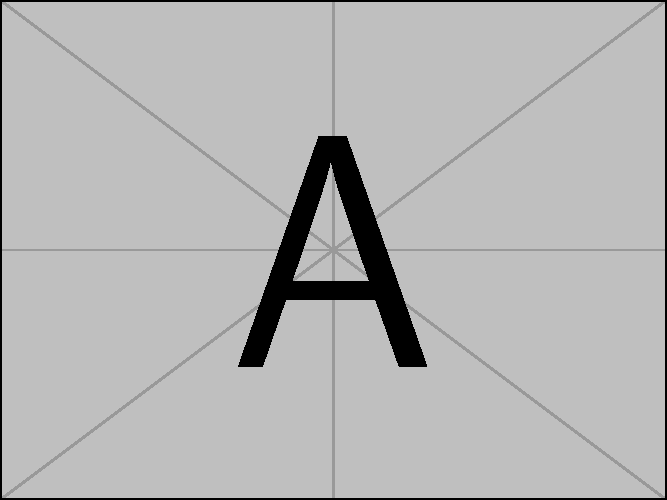
\includegraphics[width=0.5\linewidth]{example-image-a.pdf}
%   \caption*{国外的期刊习惯将图表的标题和说明文字写成一段,需要改写为标题只含图表的名称,其他说明文字以注释方式写在图表下方,或者写在正文中。}
%   \caption{示例图片标题}
%   \label{fig:example}
% \end{figure}

% 若图或表中有附注,采用英文小写字母顺序编号,附注写在图或表的下方。
% 国外的期刊习惯将图表的标题和说明文字写成一段,需要改写为标题只含图表的名称,其他说明文字以注释方式写在图表下方,或者写在正文中。

% 如果一个图由两个或两个以上分图组成时,各分图分别以 (a)、(b)、(c)...... 作为图序,并须有分图题。
% 推荐使用 \pkg{subcaption} 宏包来处理, 比如图~\ref{fig:subfig-a} 和图~\ref{fig:subfig-b}。

% \begin{figure}
%   \centering
%   \subcaptionbox{分图 A\label{fig:subfig-a}}
%     {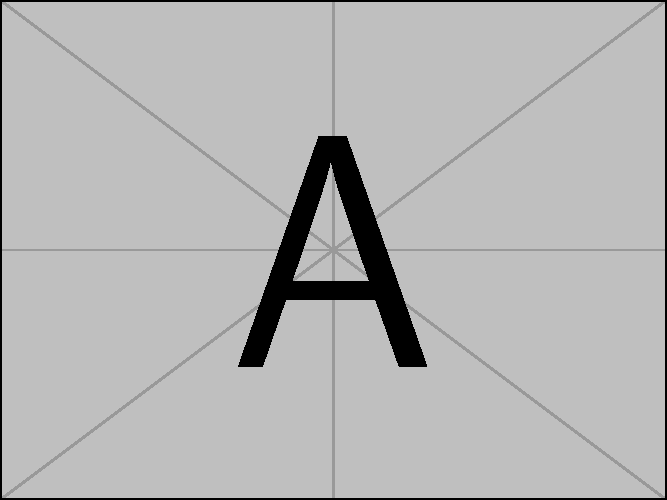
\includegraphics[width=0.35\linewidth]{example-image-a.pdf}}
%   \subcaptionbox{分图 B\label{fig:subfig-b}}
%     {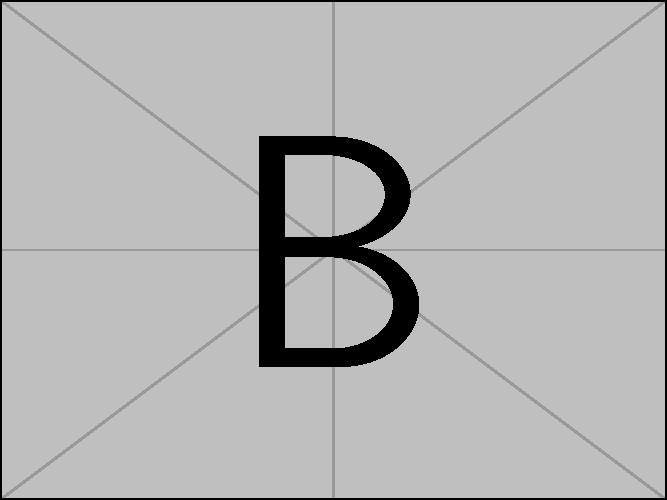
\includegraphics[width=0.35\linewidth]{example-image-b.pdf}}
%   \caption{多个分图的示例}
%   \label{fig:multi-image}
% \end{figure}



% \section{表格}

% 表应具有自明性。为使表格简洁易读,尽可能采用三线表,如表~\ref{tab:three-line}。
% 三条线可以使用 \pkg{booktabs} 宏包提供的命令生成。

% \begin{table}
%   \centering
%   \caption{三线表示例}
%   \begin{tabular}{ll}
%     \toprule
%     文件名          & 描述                         \\
%     \midrule
%     thuthesis.dtx   & 模板的源文件,包括文档和注释 \\
%     thuthesis.cls   & 模板文件                     \\
%     thuthesis-*.bst & BibTeX 参考文献表样式文件    \\
%     \bottomrule
%   \end{tabular}
%   \label{tab:three-line}
% \end{table}

% 表格如果有附注,尤其是需要在表格中进行标注时,可以使用 \pkg{threeparttable} 宏包。
% 研究生要求使用英文小写字母 a、b、c……顺序编号,本科生使用圈码 ①、②、③……编号。

% \begin{table}
%   \centering
%   \begin{threeparttable}[c]
%     \caption{带附注的表格示例}
%     \label{tab:three-part-table}
%     \begin{tabular}{ll}
%       \toprule
%       文件名                 & 描述                         \\
%       \midrule
%       thuthesis.dtx\tnote{a} & 模板的源文件,包括文档和注释 \\
%       thuthesis.cls\tnote{b} & 模板文件                     \\
%       thuthesis-*.bst        & BibTeX 参考文献表样式文件    \\
%       \bottomrule
%     \end{tabular}
%     \begin{tablenotes}
%       \item [a] 可以通过 xelatex 编译生成模板的使用说明文档;
%         使用 xetex 编译 \file{thuthesis.ins} 时则会从 \file{.dtx} 中去除掉文档和注释,得到精简的 \file{.cls} 文件。
%       \item [b] 更新模板时,一定要记得编译生成 \file{.cls} 文件,否则编译论文时载入的依然是旧版的模板。
%     \end{tablenotes}
%   \end{threeparttable}
% \end{table}

% 如某个表需要转页接排,可以使用 \pkg{longtable} 宏包,需要在随后的各页上重复表的编号。
% 编号后跟表题(可省略)和“(续)”,置于表上方。续表均应重复表头。

% \begin{longtable}{cccc}
%     \caption{跨页长表格的表题} \\
%     \toprule
%     表头 1 & 表头 2 & 表头 3 & 表头 4 \\
%     \midrule
%   \endfirsthead
%     \caption[]{跨页长表格的表题(续)} \\
%     \toprule
%     表头 1 & 表头 2 & 表头 3 & 表头 4 \\
%     \midrule
%   \endhead
%     \bottomrule
%   \endfoot
%   Row 1  & & & \\
%   Row 2  & & & \\
%   Row 3  & & & \\
%   Row 4  & & & \\
%   Row 5  & & & \\
%   Row 6  & & & \\
%   Row 7  & & & \\
%   Row 8  & & & \\
%   Row 9  & & & \\
%   Row 10 & & & \\
% \end{longtable}



% \section{算法}

% 算法环境可以使用 \pkg{algorithms} 或者 \pkg{algorithm2e} 宏包。

% \renewcommand{\algorithmicrequire}{\textbf{输入:}\unskip}
% \renewcommand{\algorithmicensure}{\textbf{输出:}\unskip}

% \begin{algorithm}
%   \caption{Calculate $y = x^n$}
%   \label{alg1}
%   \small
%   \begin{algorithmic}
%     \REQUIRE $n \geq 0$
%     \ENSURE $y = x^n$

%     \STATE $y \leftarrow 1$
%     \STATE $X \leftarrow x$
%     \STATE $N \leftarrow n$

%     \WHILE{$N \neq 0$}
%       \IF{$N$ is even}
%         \STATE $X \leftarrow X \times X$
%         \STATE $N \leftarrow N / 2$
%       \ELSE[$N$ is odd]
%         \STATE $y \leftarrow y \times X$
%         \STATE $N \leftarrow N - 1$
%       \ENDIF
%     \ENDWHILE
%   \end{algorithmic}
% \end{algorithm}
